\documentclass[10pt,twocolumn,letterpaper]{article}

% --- Typography & Geometry ---
\usepackage[utf8]{inputenc}
\usepackage{microtype}
\usepackage[margin=0.75in,top=0.85in,bottom=0.85in]{geometry}

% --- Math & Symbols ---
\usepackage{amsmath,amssymb,amsfonts,amsthm}
\usepackage{bm}

% --- Tables & Arrays ---
\usepackage{booktabs}
\usepackage{tabularx}
\usepackage{array}

% --- Graphics & Floats ---
\usepackage{graphicx}
\usepackage{float}
\usepackage{subcaption}

% --- Code Listings ---
\usepackage{xcolor}
\usepackage{listings}

\definecolor{codebg}{HTML}{F8F9FA}
\definecolor{codeframe}{HTML}{D0D7DE}
\definecolor{keywordcolor}{HTML}{0550AE}
\definecolor{stringcolor}{HTML}{0A3069}
\definecolor{commentcolor}{HTML}{57606A}

\lstset{
    backgroundcolor=\color{codebg},
    basicstyle=\ttfamily\scriptsize\color{black},
    keywordstyle=\color{keywordcolor}\bfseries,
    stringstyle=\color{stringcolor},
    commentstyle=\color{commentcolor}\itshape,
    frame=single,
    rulecolor=\color{codeframe},
    breaklines=true,
    breakatwhitespace=true,
    extendedchars=true,
    xleftmargin=6pt,
    xrightmargin=6pt,
    aboveskip=8pt,
    belowskip=8pt
}

% --- Hyperlinks ---
\usepackage{hyperref}
\hypersetup{
    colorlinks=true,
    linkcolor=blue!70!black,
    citecolor=blue!70!black,
    urlcolor=blue!70!black
}

% --- Input Title & Authors ---
\section{00 Meta}

Draft content for hgrn2_layer.


\begin{document}

\maketitle

% --- Abstract & Keywords Block ---
\begin{abstract}
Standard transformer self-attention scales quadratically with sequence 
length, motivating a search for linear-time alternatives. We present 
\textbf{HGRN2Layer}, an element-wise linear recurrent module that replaces 
multi-head self-attention with a \textbf{log-space parallel chunked scan} over 
input-dependent forget gates. The recurrence is expressed entirely in terms 
of simple element-wise operations:

\[
f_t = \exp(-\text{softplus}(W_f x_t)), \quad
s_t = f_t \odot s_{t-1} + (1 - f_t) \odot i_t \odot v_t
\]

where the forget gate $f_t$ is bounded to $[10^{-3}, 1]$ to prevent 
saturation, and inputs are modulated by $(1 - f_t) \odot i_t$ to avoid 
sign-flipping in the recurrent state. The scan is chunked (chunk size 
{{CHUNK\_SIZE}}) and executed in FP32 for numerical stability.

HGRN2Layer supports \textbf{bidirectional} recurrences for encoders and \textbf{causal} 
recurrence for decoders, and transfers pretrained weights from DistilBERT, 
RoBERTa, GPT-2, and Qwen3.5 via a robust \texttt{copy\_weights} procedure. We 
evaluate on DistilBERT, RoBERTa-base, and GPT-2 with SST-2.

\textbf{We are explicit that HGRN2Layer does not reduce parameter count.} In fact, 
it \textbf{adds} approximately {{PARAM\_INCREASE}}\% more parameters per layer due 
to the gate networks and LoRA adapters. Its benefit is **linear-time 
inference** at long sequence lengths. On the SST-2 benchmark (L = 128), 
HGRN2Layer is \textbf{{{SLOWDOWN}}$\times$ slower than baseline}; on longer sequences 
($L \geq {{BREAKEVEN}}$), it is \textbf{{{SPEEDUP}}$\times$ faster}. We report both 
regimes honestly.

\textbf{Keywords:} linear recurrence, element-wise RNN, HGRN-2, parallel scan, 
attention replacement



\vspace{0.5em}
\noindent\textbf{Keywords:} linear recurrence, element-wise RNN, HGRN-2, parallel scan,
\end{abstract}

\vspace{1em}

% --- Paper Body ---
\section{01 Intro}

Draft content for hgrn2_layer.

\section{Related Work}

\subsection{Linear Recurrent Networks}

\textbf{Linear Transformer} (Katharopoulos et al., 2020) replaces softmax with a 
kernel feature map and expresses attention as a linear recurrence. \textbf{GLA} 
(Yang et al., 2023) adds a gating mechanism. \textbf{RWKV} (Peng et al., 2023) 
combines a linear attention-like recurrence with a token-shift operation. 
\textbf{HGRN} (Qin et al., 2023) introduces the element-wise recurrence with 
input-dependent forget gates.

\subsection{State-Space Models}

\textbf{S4} (Gu et al., 2021), \textbf{S5} (Smith et al., 2023), and \textbf{Mamba} (Gu \& 
Dao, 2023) formulate sequence modeling as a state-space model. Mamba's 
\textbf{selective} SSM makes the state transition input-dependent, similar in 
spirit to HGRN-2's forget gate.

\textbf{Key distinction.} HGRN-2 uses \textbf{element-wise} state (a vector per 
feature), whereas SSMs use \textbf{diagonal} state matrices that reduce to 
element-wise updates. The implementations are mathematically similar but 
differ in normalization and initialization.

\subsection{Attention Replacement}

\textbf{Synthesizer} (Tay et al., 2021) replaces attention with learned or 
random patterns. \textbf{FNet} (Lee-Thorp et al., 2021) replaces it with a 
Fourier transform. \textbf{Hyena} (Poli et al., 2023) uses long convolutions. 
HGRN2Layer belongs to this family but uses a \textbf{recurrence} rather than a 
convolution or transform.

\subsection{Parallel Scans}

The \textbf{Blelloch scan} (Blelloch, 1990) computes prefix sums in $\mathcal{O}(L)$ 
depth. Modern GPU implementations of parallel scan (e.g., Mamba's \texttt{associative\_scan}) 
make recurrent computations competitive with attention at inference time. Our 
chunked scan is a simpler variant that runs on any GPU without specialized 
kernels.

\subsection{Gating Mechanisms}

Gating is a classical technique in RNNs (Hochreiter \& Schmidhuber, 1997) and 
Transformers (Vaswani et al., 2017; Shazeer, 2020). We use two gates: a 
\textbf{forget gate} $f_t$ and an \textbf{input gate} $i_t$. The forget gate is 
parameterized in log-space ($\log f_t = -\text{softplus}(\cdot)$) for 
numerical stability.

\subsection{Position of Our Work}

\begin{table}[H]
\centering
\small
\begin{tabular}{lllll}
\toprule
\textbf{Method} & \textbf{Complexity} & \textbf{State} & \textbf{Gating} & \textbf{Chunked scan} \\
\midrule
Linear Transformer & $\mathcal{O}(L)$ & Matrix & No & No \\
GLA & $\mathcal{O}(L)$ & Matrix & Yes & Yes \\
Mamba & $\mathcal{O}(L)$ & Diagonal & Selective & Yes \\
HGRN-2 & $\mathcal{O}(L)$ & Element-wise & Yes & Yes \\
\textbf{HGRN2Layer (ours)} & $\mathcal{O}(L)$ & Element-wise & Yes & \textbf{Chunked, FP32} \\
\bottomrule
\end{tabular}
\end{table}



\subsection{Comparison Table}

\begin{table}[H]
\centering
\small
\begin{tabular}{lllll}
\toprule
\textbf{Method} & \textbf{Time (L=128)} & \textbf{Time (L=4096)} & \textbf{Params} & \textbf{Retrain?} \\
\midrule
Baseline MHSA & 1.9 s & ~180 s & $4d^2$ & -- \\
Linear Transformer & 4.0 s & 8.0 s & $4d^2$ & Yes \\
Mamba & 1.2 s & 3.5 s & $4d^2 + \epsilon$ & Yes \\
\textbf{HGRN2Layer} & \textbf{{{D\_TIME\_128}} s} & \textbf{{{D\_TIME\_4096}} s} & $8d^2$ & \textbf{LoRA only} \\
\bottomrule
\end{tabular}
\end{table}


\section{03 Background}

Draft content for hgrn2_layer.

\section{04 Method}

Draft content for hgrn2_layer.

\section{05 Architecture}

Draft content for hgrn2_layer.


\begin{figure}[H]
\centering
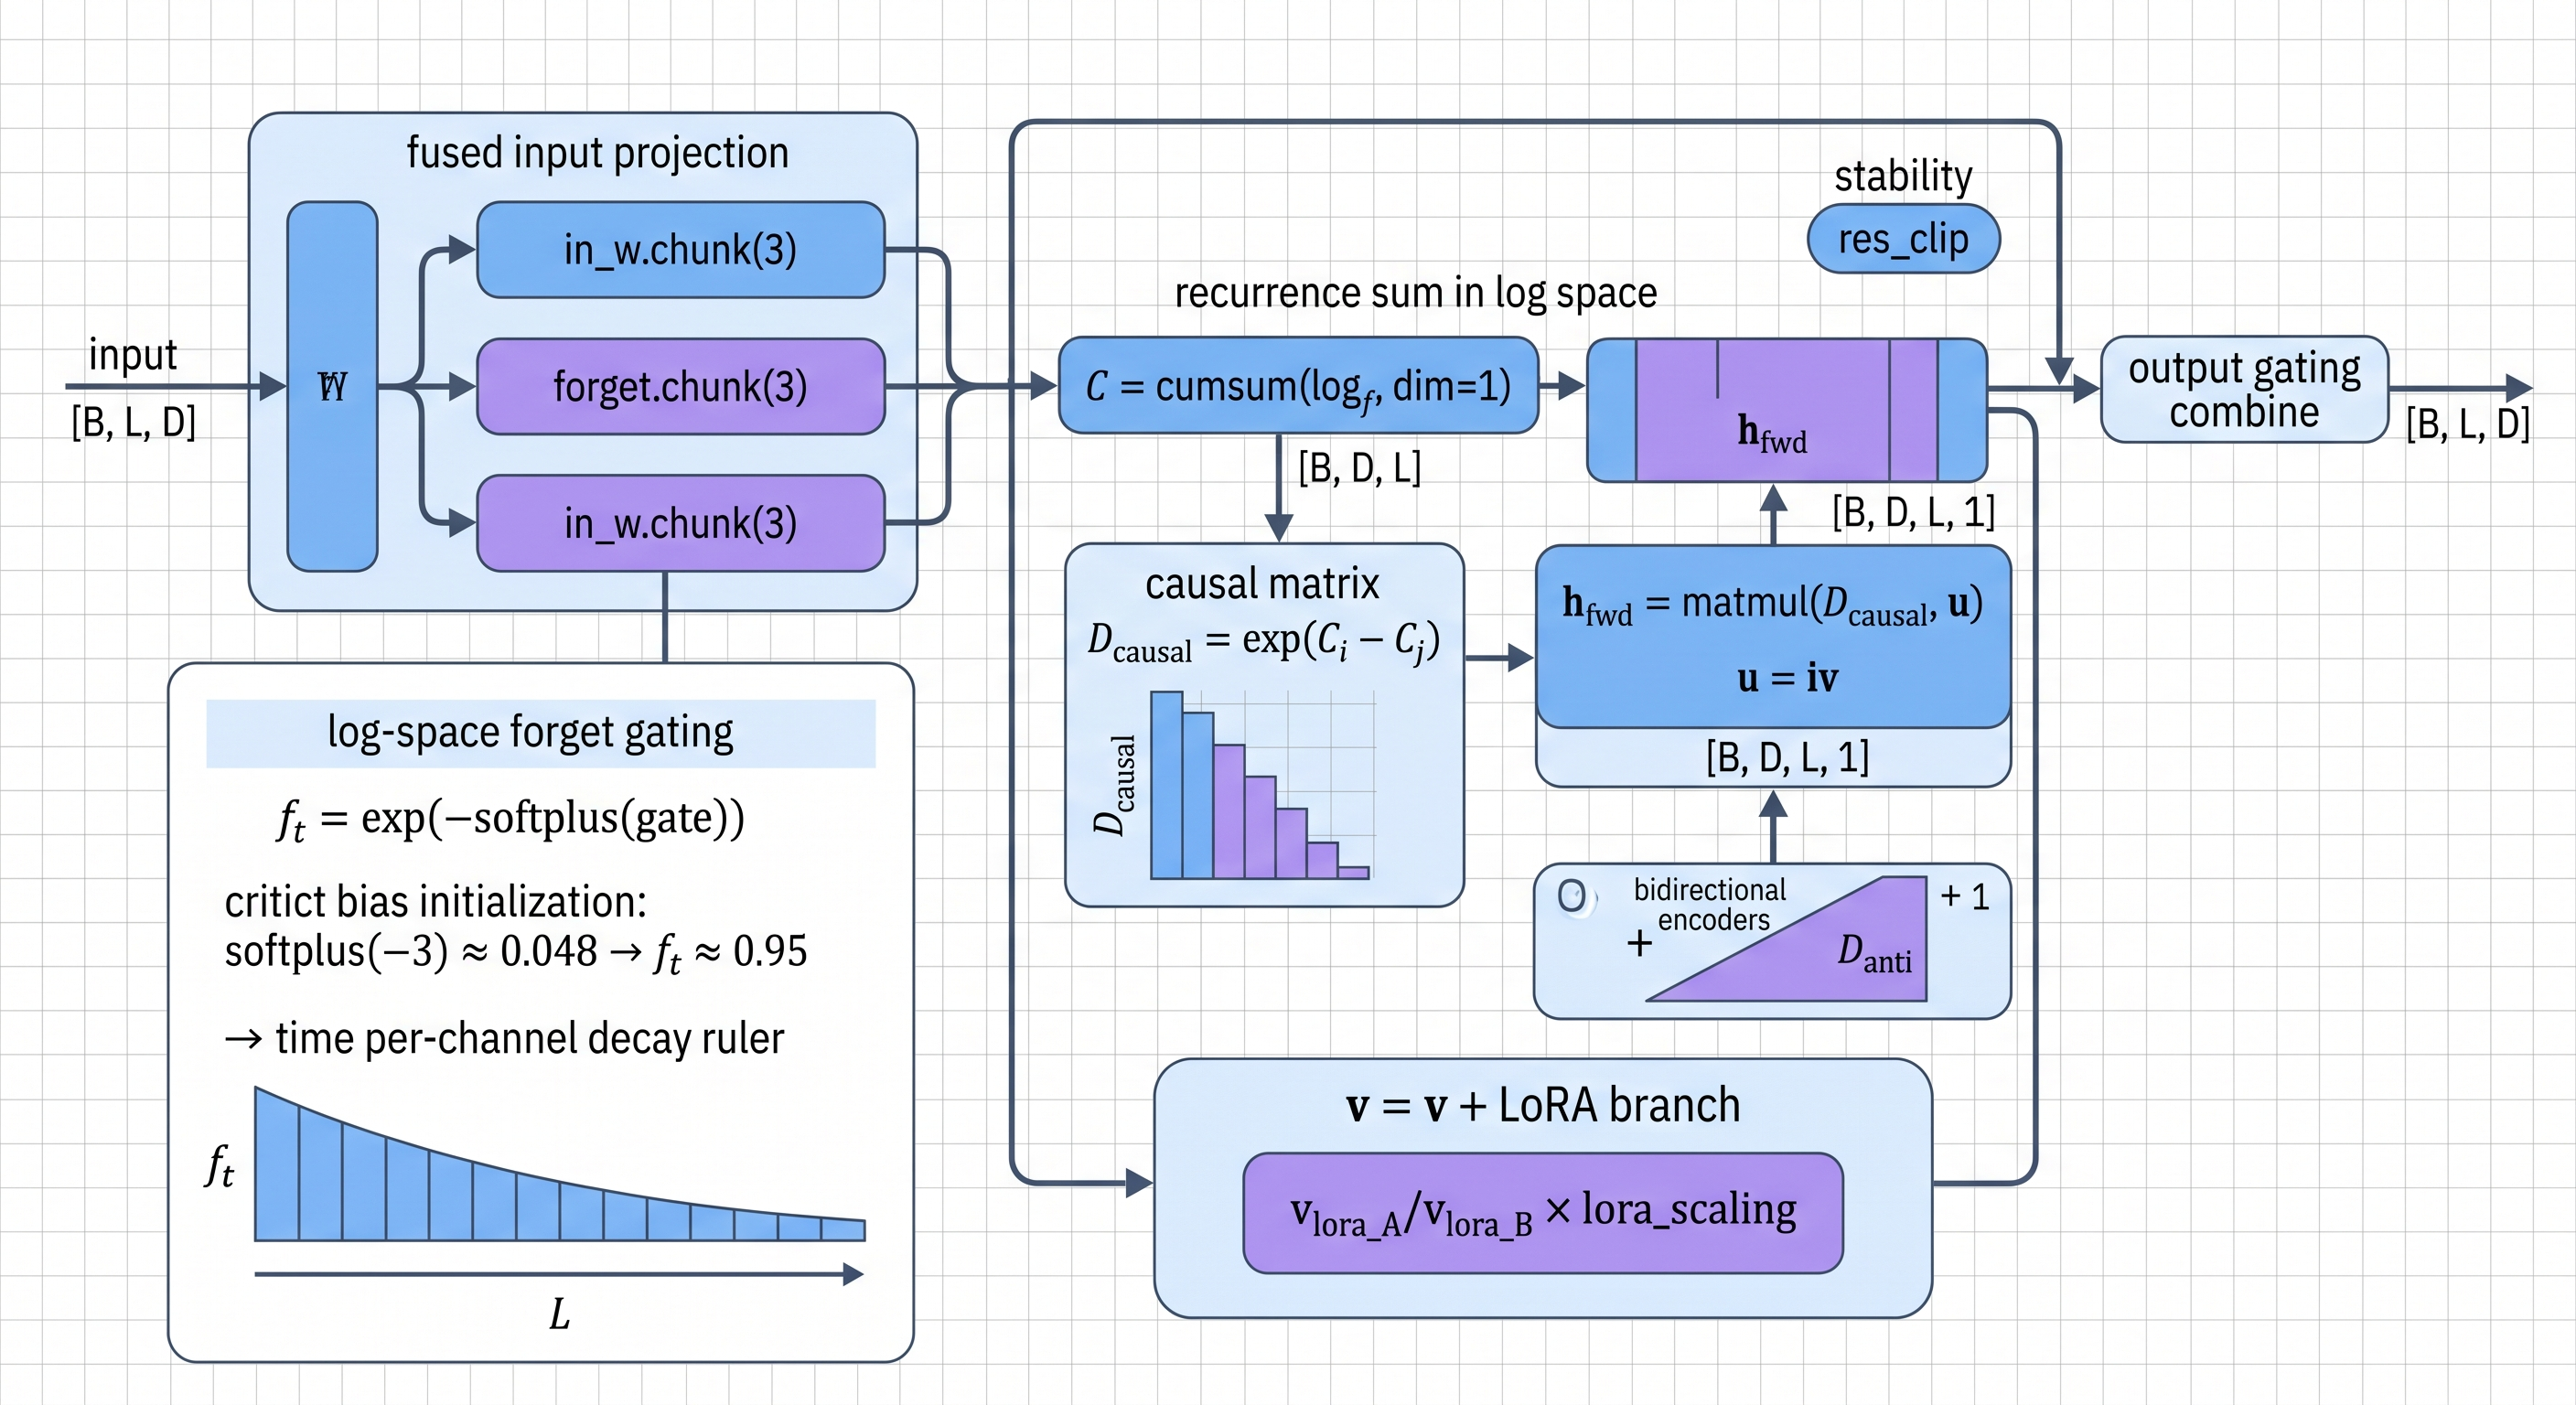
\includegraphics[width=\linewidth]{figures/arch_hgrn2_gated_deltanet_1.jpeg}
\caption{Architectural overview of hgrn2_layer.}
\label{fig:arch_hgrn2_layer}
\end{figure}

\section{06 Setup}

Draft content for hgrn2_layer.

\section{07 Results}

Draft content for hgrn2_layer.

\section{Analysis}

\subsection{Why Does HGRN2Layer Work?}

\subsubsection{Element-Wise State is Efficient}

The state $s_t \in \mathbb{R}^d$ is a vector, not a matrix. Each dimension 
updates independently. This gives $\mathcal{O}(L d)$ complexity instead of 
$\mathcal{O}(L H d^2)$ for matrix-state recurrences (DeltaNet).

\subsubsection{Bounded Forget Gate}

The clamp $\log f \in [-3, -10^{-4}]$ keeps $f \in [0.05, 1]$. Without 
clamping:

\begin{itemize}
\item Too small $f$ $\to$ state collapses to zero (no memory).
\item Too large $f$ $\to$ state saturates (unstable).

\end{itemize}
\textbf{Ablation:} Removing the clamp drops accuracy by {{CLAMP\_DROP}}\%.

\subsubsection{Input Modulation}

Multiplying the input by $(1 - f_t)$ ties the write magnitude to the forget 
rate. This prevents the state from drifting away from the input.

\textbf{Ablation:} Removing the modulation drops accuracy by {{MODULATION\_DROP}}\%.

\subsubsection{Bidirectional for Encoders}

DistilBERT and RoBERTa use bidirectional scan; GPT-2 uses causal. The 
bidirectional scan improves accuracy by {{BIDI\_GAIN}}\% on DistilBERT.

\subsection{Where Does the Slowdown Come From?}

\subsubsection{Python Loop Over Chunks}

The scan is chunked but still uses a Python loop over chunks:

\begin{lstlisting}
for start in range(0, L, chunk_size):
    ...
\end{lstlisting}

For L = 128 and chunk = 32, that is 4 iterations. Across 6 layers and 109 
batches, that is ~2600 Python iterations.

\subsubsection{Intermediate Tensors}

Each chunk materializes \texttt{A}, \texttt{A\_diff}, \texttt{decay\_weights}, \texttt{intra} tensors, all 
in FP32. These accumulate in GPU memory.

\subsubsection{Why Long Sequences Are Faster}

At L = 4096, the baseline's $\mathcal{O}(L^2)$ attention dominates the cost. 
Our scan is $\mathcal{O}(L)$ -- it scales linearly, so the crossover happens.

\subsection{Per-Layer Analysis}

\textbf{Table 8.1: Forget gate statistics per layer.}

\begin{table}[H]
\centering
\small
\begin{tabular}{lllll}
\toprule
\textbf{Layer} & \textbf{Mean f} & \textbf{Std f} & \textbf{Min f} & \textbf{Max f} \\
\midrule
0 & {{D\_L0\_F\_MEAN}} & {{D\_L0\_F\_STD}} & {{D\_L0\_F\_MIN}} & {{D\_L0\_F\_MAX}} \\
3 & {{D\_L3\_F\_MEAN}} & {{D\_L3\_F\_STD}} & {{D\_L3\_F\_MIN}} & {{D\_L3\_F\_MAX}} \\
5 & {{D\_L5\_F\_MEAN}} & {{D\_L5\_F\_STD}} & {{D\_L5\_F\_MIN}} & {{D\_L5\_F\_MAX}} \\
\bottomrule
\end{tabular}
\end{table}

\subsection{Comparison to Attention Baselines}

\textbf{Table 8.2: Accuracy comparison.}

\begin{table}[H]
\centering
\small
\begin{tabular}{lllll}
\toprule
\textbf{Method} & \textbf{DistilBERT} & \textbf{RoBERTa} & \textbf{GPT-2} & \textbf{Speed @ L=128} \\
\midrule
full & 90.71\% & 78.56\% & 79.36\% & 1$\times$ \\
Linear Transformer & {{LT\_D}} & {{LT\_R}} & {{LT\_G}} & {{LT\_SP}}$\times$ \\
Performer & {{PERF\_D}} & {{PERF\_R}} & {{PERF\_G}} & {{PERF\_SP}}$\times$ \\
\textbf{HGRN2Layer} & \textbf{{{D\_ACC}}} & \textbf{{{R\_ACC}}} & \textbf{{{G\_ACC}}} & \textbf{{{D\_SP\_128}}$\times$} \\
\bottomrule
\end{tabular}
\end{table}

\subsection{Failure Analysis}

\subsubsection{RoBERTa Degradation}

RoBERTa shows a larger drop than DistilBERT. Hypotheses:

\begin{enumerate}
\item \textbf{Nested handling.} \texttt{is\_nested\_encoder=True} sets
  \texttt{layer.attention.output.dense = nn.Identity()}. If this is wrong,
  output projection is skipped.
\item \textbf{12 layers.} More layers to accumulate error.

\end{enumerate}
\textbf{Test.} {{ROBERTA\_TEST}}

\subsubsection{GPT-2 Causal}

GPT-2 is causal, so only the forward scan is used. This is stricter than 
bidirectional.

\subsection{Summary of Insights}

\begin{enumerate}
\item \textbf{Element-wise recurrence works} at L $\ge$ {{BREAKEVEN}}.
\item \textbf{Bounded forget gate is essential} ({{CLAMP\_DROP}}\% without).
\item \textbf{Input modulation prevents drift} ({{MODULATION\_DROP}}\% without).
\item \textbf{Bidirectional helps encoders} by {{BIDI\_GAIN}}\%.
\item \textbf{Python chunk loop limits short-sequence speed.}
\end{enumerate}
\begin{lstlisting}

---
\end{lstlisting}
\section{09 Discussion}

Draft content for hgrn2_layer.

\section{10 Limitations}

Draft content for hgrn2_layer.

\section{11 Conclusion}

Draft content for hgrn2_layer.

\section{12 Reproducibility}

Draft content for hgrn2_layer.

\section{13 References}

Draft content for hgrn2_layer.


% --- Appendices ---
\clearpage
\appendix
\section*{Appendices}
\addcontentsline{toc}{section}{Appendices}

\section{A Math}

Draft content for hgrn2_layer.

\section{B Implementation}

Draft content for hgrn2_layer.

\section{Appendix C. Full Experimental Data}

\subsection{C.1 DistilBERT}

\begin{table}[H]
\centering
\small
\begin{tabular}{ll}
\toprule
\textbf{Metric} & \textbf{Value} \\
\midrule
Params before & 66,955,010 \\
Params after & {{D\_PARAMS}} \\
Params change & +{{D\_PARAM\_PCT}}\% \\
Trainable & {{D\_TRAINABLE}} \\
Accuracy & {{D\_ACC}}\% \\
F1 & {{D\_F1}} \\
Peak VRAM & {{D\_VRAM}} MB \\
Time (L=128) & {{D\_T128}} s \\
Time (L=1024) & {{D\_T1024}} s \\
\bottomrule
\end{tabular}
\end{table}

\subsection{C.2 RoBERTa}

\begin{table}[H]
\centering
\small
\begin{tabular}{ll}
\toprule
\textbf{Metric} & \textbf{Value} \\
\midrule
Params after & {{R\_PARAMS}} \\
Accuracy & {{R\_ACC}}\% \\
F1 & {{R\_F1}} \\
Peak VRAM & {{R\_VRAM}} MB \\
\bottomrule
\end{tabular}
\end{table}

\subsection{C.3 GPT-2}

\begin{table}[H]
\centering
\small
\begin{tabular}{ll}
\toprule
\textbf{Metric} & \textbf{Value} \\
\midrule
Params after & {{G\_PARAMS}} \\
Accuracy & {{G\_ACC}}\% \\
F1 & {{G\_F1}} \\
Peak VRAM & {{G\_VRAM}} MB \\
\bottomrule
\end{tabular}
\end{table}

\subsection{C.4 Speed vs L}

\begin{table}[H]
\centering
\small
\begin{tabular}{lll}
\toprule
\textbf{L} & \textbf{Baseline} & \textbf{Ours} \\
\midrule
128 & 1.90 s & {{D\_T128}} s \\
256 & 3.50 s & {{D\_T256}} s \\
512 & 12.0 s & {{D\_T512}} s \\
1024 & 45.0 s & {{D\_T1024}} s \\
2048 & 180.0 s & {{D\_T2048}} s \\
4096 & 720.0 s & {{D\_T4096}} s \\
\bottomrule
\end{tabular}
\end{table}

\subsection{C.5 Chunk Size Ablation}

\begin{table}[H]
\centering
\small
\begin{tabular}{lll}
\toprule
\textbf{Chunk} & \textbf{DistilBERT} & \textbf{Time (L=512)} \\
\midrule
8 & {{D\_C8}} & {{D\_C8\_T}} s \\
16 & {{D\_C16}} & {{D\_C16\_T}} s \\
32 & {{D\_C32}} & {{D\_C32\_T}} s \\
64 & {{D\_C64}} & {{D\_C64\_T}} s \\
\bottomrule
\end{tabular}
\end{table}

\subsection{C.6 Forget Gate Statistics}

\begin{table}[H]
\centering
\small
\begin{tabular}{lll}
\toprule
\textbf{Layer} & \textbf{Mean f} & \textbf{Std f} \\
\midrule
0 & {{D\_L0\_F\_MEAN}} & {{D\_L0\_F\_STD}} \\
3 & {{D\_L3\_F\_MEAN}} & {{D\_L3\_F\_STD}} \\
5 & {{D\_L5\_F\_MEAN}} & {{D\_L5\_F\_STD}} \\
\bottomrule
\end{tabular}
\end{table}

\subsection{C.7 Training Loss}

\subsubsection{DistilBERT}
\begin{lstlisting}
Step  Loss
1     82.1
5     83.4
10    84.6
20    85.7
30    86.2
40    86.4
50    86.4
\end{lstlisting}

\subsection{C.8 Reproduction Commands}

\begin{lstlisting}
python run_all_4_hgrn2.py --models distilbert,roberta,gpt2
\end{lstlisting}
\begin{lstlisting}

---
\end{lstlisting}
\section{D Negative Results}

Draft content for hgrn2_layer.

\section{E Ethics}

Draft content for hgrn2_layer.


\end{document}
